W całej pracy jako przestrzeń rozumiemy przestrzeń metryczną i ośrodkową. 
\section{Podstawowe definicje}
Zanim przejdziemy do pokazania definicji wymiaru pokryciowego, zacznijmy od przypomnienia i wprowadzenia kilku definicji pomocniczych.

\begin{defi}
    Jeżeli przestrzeń $X$ spełnia:
    dla każdej pary zbiorów domkniętych $A, B \subset X$ spełniających $A\cap B=\emptyset$, istnieją takie otwarte zbiory $U, V\subset X$, że $A\subset U$, $B\subset V$, $U\cap V=\emptyset$, to powiemy że $X$ jest przestrzenią \emph{normalną}.
\end{defi}
Podana własność często jest również nazywana własnością \emph{T4}. Dla przypomnienia, własnością \emph{T2}, czyli przestrzeń Hausdorffa, nazywamy możliwość oddzielenia dwóch punktów przez otoczenia otwarte, a własnością \emph{T3}, czyli przestrzeń regularną, możliwość oddzielenia punktów od zbiorów domkniętych przez otoczenia otwarte. 
\begin{defi}
    Powiemy, że przestrzeń jest \emph{zwarta}, jeżeli z każdego otwartego pokrycia możemy wybrać podpokrycie skończone.
\end{defi}

\begin{defi}
    Pokrycie $\mathcal{B}$ jest \emph{wpisaniem} pokrycia $\mathcal{A}$ tej samej przestrzeni $X$, jeżeli dla każdego $B\in \mathcal{B}$ istnieje $A\in \mathcal{A}$, takie że $B\subset A$.
    \begin{figure}[H]
        \centering
        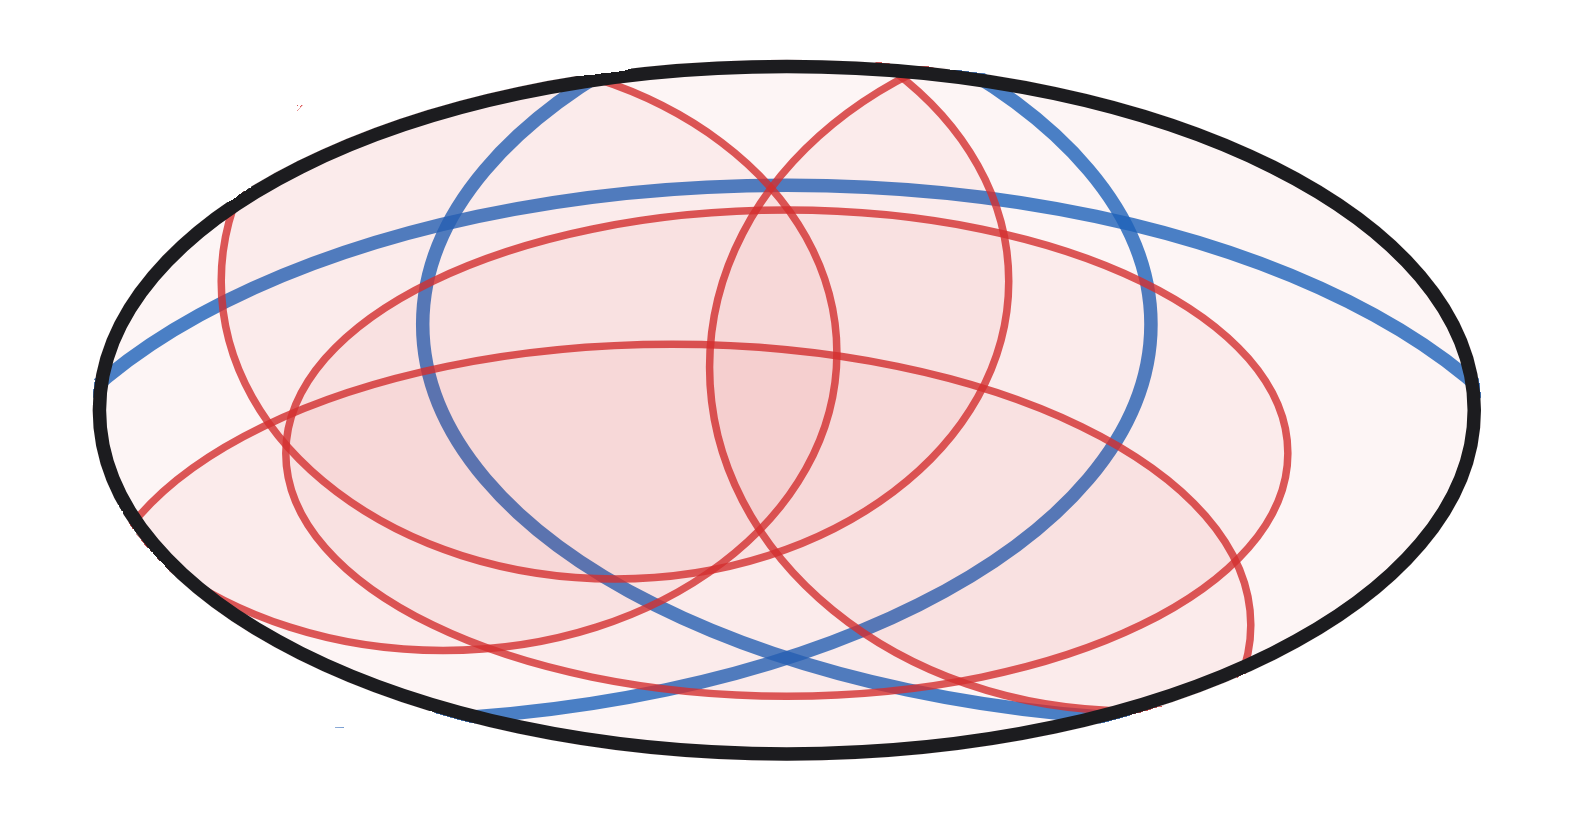
\includegraphics[width=0.5\textwidth]{pictures/wpisanie_przy.png}
        \caption{wpisanie}
        \label{fig:wpis}
    \end{figure}
\end{defi}
\begin{defi}
    \emph{Zwężeniem} pokrycia $\{A_s\}_{s\in S}$ przestrzeni $X$ nazwiemy pokrycie $\{B_s\}_{s\in S}$ przestrzeni $X$ spełniające $\forall_{s\in S} B_s \subset A_s$.
    \begin{figure}[H]
        \centering
        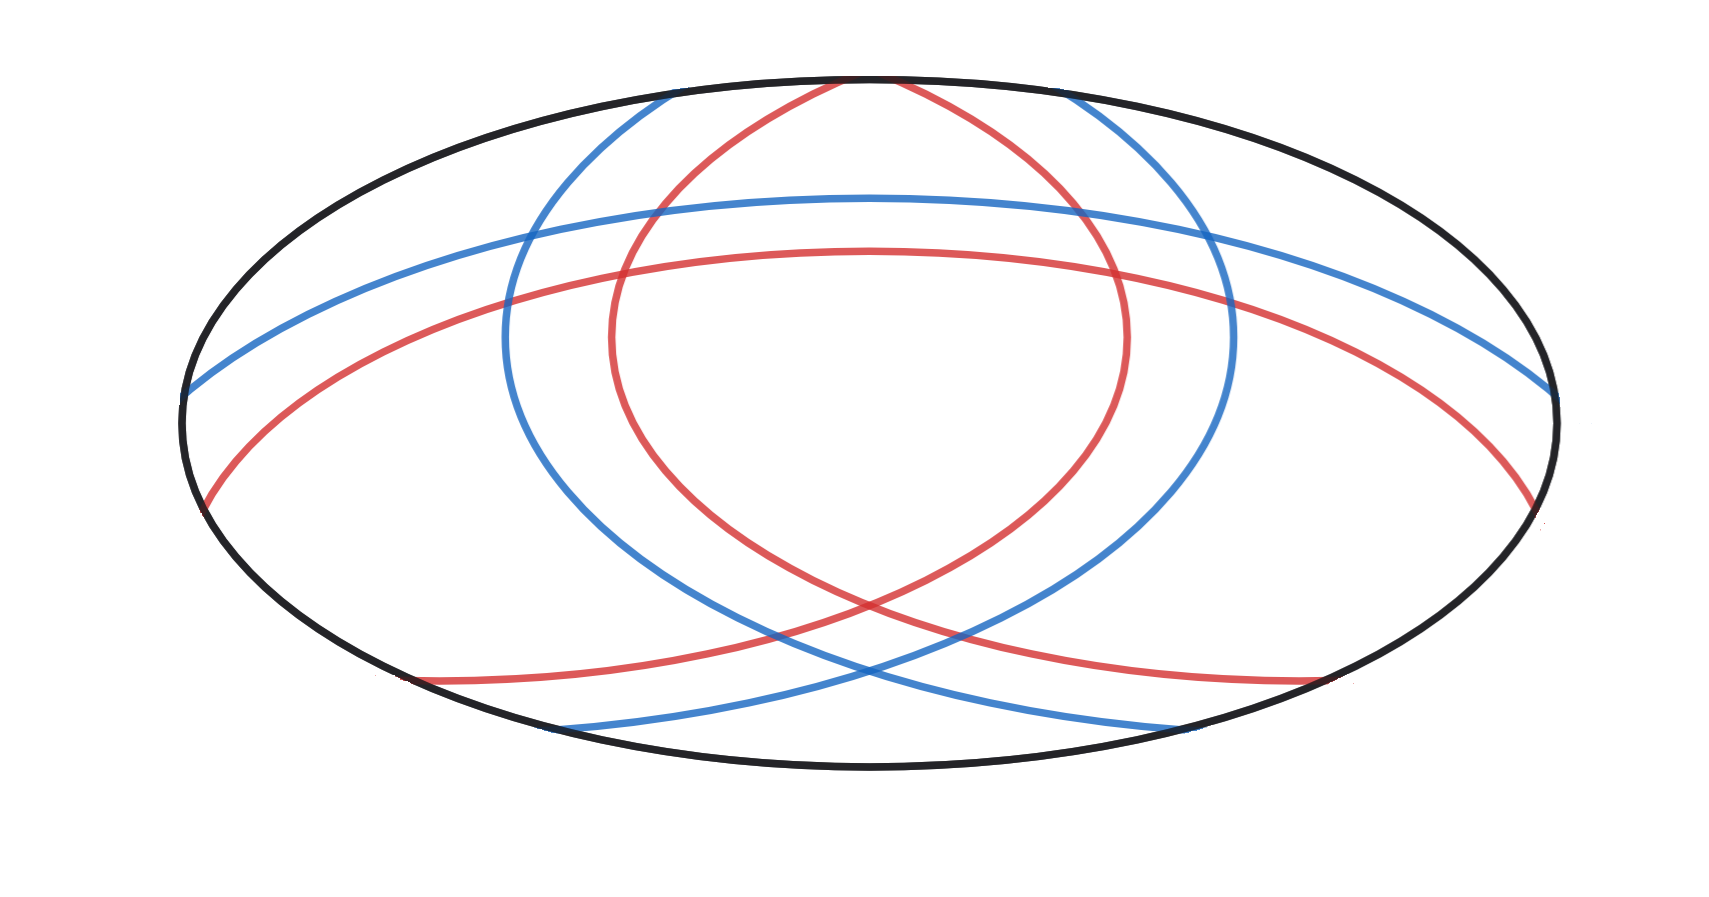
\includegraphics[width=0.5\textwidth]{pictures/zwerzenie_przy.png}
        \caption{zwężenie}
        \label{fig:zwerz}
    \end{figure}
\end{defi}
Zauważmy, że oczywiście każde zwężenie jest również wpisaniem.

% \subsection{Krotność}
Teraz zdefiniujemy pojęcie, które będzie kluczowe w definicji wymiaru pokryciowego.
\begin{defi}
    Niech $X$ będzie zbiorem a $A$ niech będzie rodziną podzbiorów $X$. Wtedy \emph{krotnością} rodziny $A$ (ozn. $\ord A$) nazwiemy największe takie całkowite $n$, że $A$ zawiera $n+1$ zbiorów z niepustym przecięciem. Gdy takie $n$ nie istnieje, powiemy że $\ord A=\infty$.  
\end{defi}
\begin{wnio}
    Dla rodziny o krotności $n$, przecięcie każdych $n+2$ parami różnych elementów jest puste.
\end{wnio}
Możemy łatwo zauważyć, że rodzina o krotności $-1$ musi zawierać jedynie zbiory puste, a rodzina o krotności 0 stwożona jest ze zbiorów parami rozłącznych, w których nie wszystkie są puste.
\\
Teraz możemy przejść do wprowadzenia naszej definicji.

\section{Wymiar Pokryciowy}
\begin{defi}    
    \emph{Wymiarem pokryciowym} przestrzeni normalnej $X$ (ozn. $\dim X)$ nazwiemy liczbę całkowitą $\geq -1$ lub $\infty$ spełniającą następujące własności:
    \begin{itemize}
        \item[(ČL1)] $\dim X\leq n$ dla $n=-1,0,1,\cdots$, jeśli dla każdego skończonego otwartego pokrycia przestrzeni $X$ istnieje skończone wpisanie krotności $\leq n$,
        \item[(ČL2)] $\dim X=n$ jeżeli zachodzą nierówności $n-1<\dim X\leq n$,
        \item[(ČL3)] $\dim X=\infty$, jeżeli dla każdego $n=-1,0,1,\ldots$ zachodzi $\dim X >n$
    \end{itemize} 
\end{defi}
\emph{ČL} pochodzi tutaj od nazwisk Čech i Lebesque, którzy, jak wspomniane było wcześniej, jako pierwsi wprowadzili definicję wymiaru pokryciowego.\\
Łatwo możemy zauważyć, że jeżeli przestrzenie $X$ i $Y$ są homeomorficzne, to oczywiście spełniają $\dim X = \dim Y$, kożystamy tutaj z własności zamknięcia homeomorfizmu na zbiory otwarte, jak również że dla wszystkich przestrzeni euklidesowych $\dim \mathbb{R}^n=n$. 
\begin{przy}
    Zobaczmy, że dla każdego pokrycia przestrzeni euklidesowej $\mathbb{R}^1\cong \mathbb{R}$, znajdziemy pokrycie postaci 
    \begin{figure}[H]
        \centering
        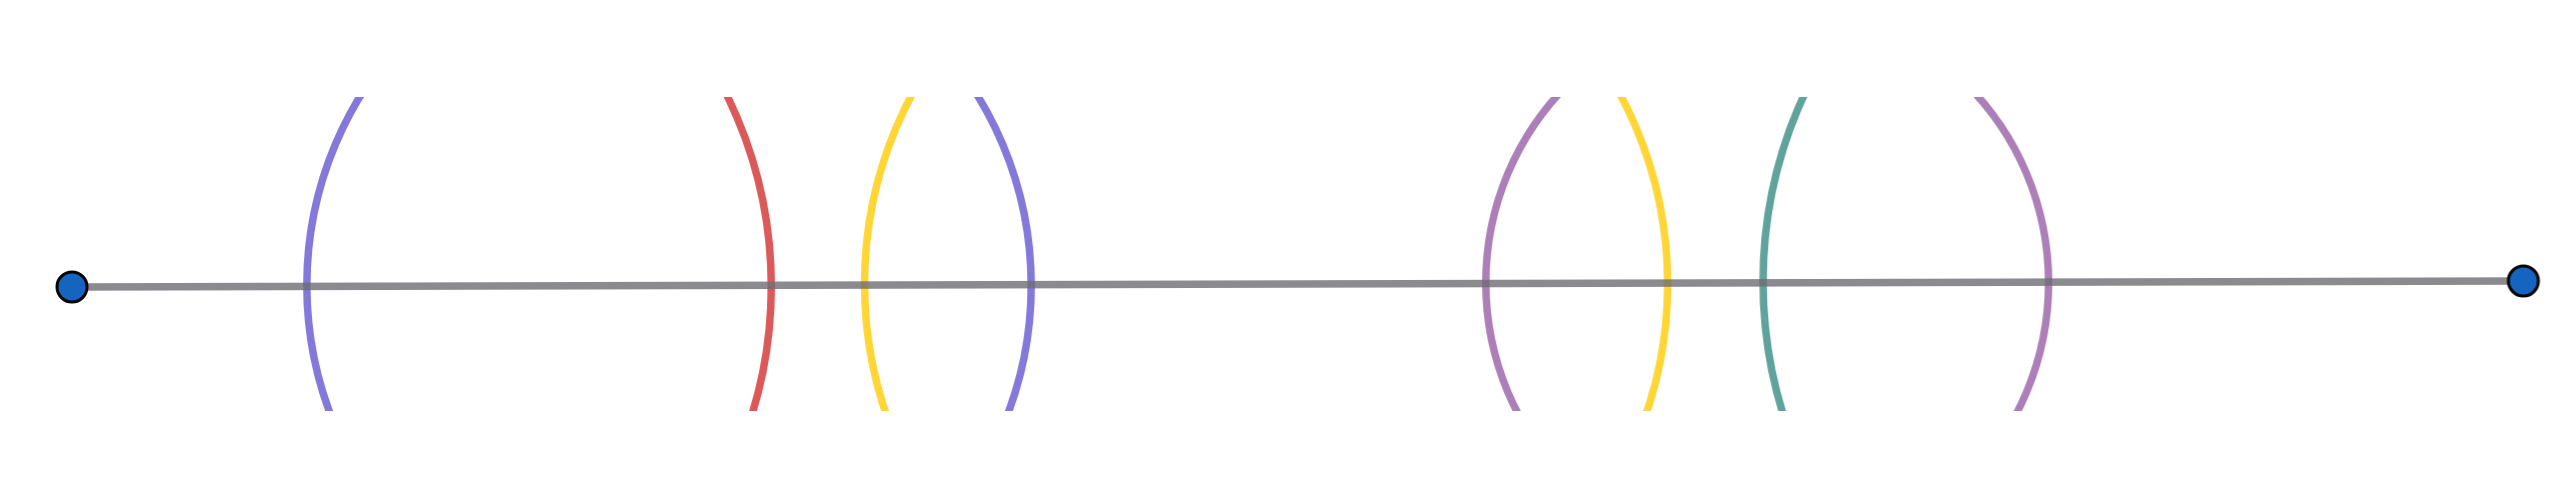
\includegraphics[width=0.8\textwidth]{pictures/wymiar_1.png}
        % \caption{wymiar}
        \label{fig:wymiar_1}
    \end{figure}
    które jest oczywiście krotności 1. 
\end{przy}
\begin{przy}
    Ewentualnie dodać przykład dla $R^2$
     \begin{figure}[H]
        \centering
        \includesvg[width=0.2\textwidth]{pictures/Refinement_on_a_planar_shape.svg}
        % \caption{zwężenie pokrycia kwadratu}
        \label{fig:wymiar_2}
    \end{figure}
    \end{przy}
\section{Twierdzenia}
Pokażemy teraz dwa twierdzenia, pierwsze mówi o tym, że zamiast szukać wpisań możemy szukać zwężeń, drugie pokazuje, że nie musimy pokazywać instnienia zwężeń dla pokryć o dowolnie dużej liczbie elementów, tylko rozważać jedynie te o ograniczonej.
\begin{twie} % 1.6.8
    Dla każdej przestrzeni normalnej $X$ NWSR:
    \begin{itemize}
        \item[(i)] wymiar pokryciowy przestrzeni $X$ jest co najwyżej $n$
        \item[(ii)] Dla każdego skończonego otwartego pokrycia $X$ możemy znaleźć otwarte wpisanie o krotności co najwyżej $n$
        \item[(iii)] Dla każdego skończonego otwartego pokrycia $X$ możemy znaleźć otwarte zwężenie o krotności co najwyżej $n$
    \end{itemize}
\end{twie}
\begin{proof}
    Zacznijmy od zauważenia, iż implikacje (i)$\Rightarrow$(ii), (ii)$\Rightarrow$(i) oraz (iii)$\Rightarrow$(i) są oczywiste, pierwsze dwie wynikają wprost z definicji wymiaru pokryciowego, w trzeciej musimy zauważyć, że każde zwężenie jest również wpisaniem. \\
    Pozostaje w takim razie pokazać implikację (ii)$\Rightarrow$(iii)\\
    Weźmy przestrzeń normalną $X$ spełniającą (ii), oraz niech $\mathcal{U}=\{U_i\}_{i=1}^k$ będzie skończonym otwartym pokryciem przestrzeni $X$. Wiemy, że istnieje $\mathcal{V}$ - otwarte wpisanie pokrycia $\mathcal{U}$ spełniające $\ord \mathcal{V}\leq n$. Teraz z tego wpisania skonstruujemy zwężenie pokrycia $\mathcal{U}$ krotności $n$.\\
    Zaczniemy od zdefiniowania przypożądkowania $i(V)$ - taki indeks z przedziału $\{1,\ldots k\}$, dla którego $V\subset U_{i(V)}$. Teraz dla każdego $i\in \{1, \ldots, k\}$ zdefiniujmy $V_i = \bigcup\{V\;|\;i=i(V)\}$. Pokażemy, że tak zdefiniowana rodzina $\tilde{\mathcal{V}}=\{V_i\}_{i=1}^k$ jest szukanym zwężeniem. \\
    Oczywiście $\forall_i\;V_i\subset U_i$ oraz $\tilde{\mathcal{V}}$ jest pokryciem przestrzeni $X$. Pozostaje więc pokazać, że $\ord \tilde{\mathcal{V}}\le n$, jednak to wynika wprost z prostej teorii zbiorów oraz $\ord\mathcal{V}\le n$ (czyli że przecięcie każdych $n+2$ parami różnych elementów $\mathcal{V}$ jest puste), co kończy dowód. 

\end{proof}

\begin{twie} %1.6.9
    Przestrzeń normalna $X$ ma wymiar pokryciowy $\dim X \leq n $ wtedy i tylko wtedy, gdy dla każdego $n+2$ elementowego otwartego pokrycia przestrzeni $X$ - $\{U_i\} _{i=1}^{n+2}$ istnieje otwarte zwężenie $ \{W_i\} _{i=1}^{n+2}$ o krotności $\ord W\le n$, spełniające $\bigcap_{i=1}^{n+2} W_i = \emptyset$.
\end{twie}
\begin{proof}
    Zauważmy, że do dowodu tego twierdzenia wystarczy pokazać, że jeżeli przestrzeń normalna $X$ ma wymiar pokryciowy większy od $n$, to jesteśmy w stanie znaleźć $\mathcal{U}=\{U_i\}_{i=1}^{n+2}$ - takie otwarte pokrycie $n+2$-elementowe, że każde jego otwarte zwężenie $\mathcal{W}=\{W_i\}_{i=1}^{n+2}$ spełnia $\bigcap\mathcal{W}\ne \emptyset$\\
    Teraz mamy $\dim X>n$, więc wiemy że możemy znaleźć takie otwarte pokrycie $\mathcal{V}=\{V_i\}_{i=1}^{k}$ przestrzeni $X$, dla którego nie istnieje otwarte zwężenie krotności $\le n$. \\
    Do tego, jeżeli $\mathcal{V}' = \{V_i'\}_{i=1}^k$ to otwarte zwężenie pokrycia $\mathcal{V}$, to spełnia ono: 
    \[V_{i_1}\cap V_{i_2} \cap \cdots \cap V_{i_m} \ne \emptyset\;\;\;\Rightarrow\;\;\;
    V'_{i_1}\cap V'_{i_2} \cap \cdots \cap V'_{i_m} \ne \emptyset\]
    Jeżeli tak nie zachodzi, to zastępujemy $\mathcal{V}$ przez $\mathcal{V'}$. Liczba różnych przecięć jest skończona, więc po skończonej liczbie podstawień ustatkujemy się (przy każdym podstawieniu eliminujemy co najmniej jedną sprzeczną implikację).\\
    Teraz, wiemy że krotność naszego pokrycia $\mathcal{V}$ spełnia $\ord\mathcal{V}>n$, więc możemy tak przeindeksować jego elementy by zachodziła własność
    \[\bigcap_{i=1}^{n+2} V_i\ne \emptyset\]
    Pokażemy, że pokrycie $\mathcal{U} = \{U_i\}_{i=1}^{n+2}$ zdefiniowane przez:
    \[U_i=V_i\;\; \mathrm{dla}\;\; i=1,2,\ldots,n+1\]
    \[U_{n+2}= \bigcup _{i=n+2}^kV_i\]
    jest szukanym pokryciem przestrzeni $X$, czyli że dla każdego otwartego zwężenia $\mathcal{W}=\{W_i\}_{i=1}^{n+2}$ pokrycia $\mathcal{U}$ zachodzi $\bigcap\mathcal{W}\ne \emptyset$.\\
    Weźmy więc dowolne zwężenie $\mathcal{W}$ pokrycia $\mathcal{U}$. Zauważmy, że
    \[\mathcal{W'}=\{W_1, W_2, \ldots, W_{n+1}, W_{n+2}\cap V_{n+2}, \ldots W_{n+2}\cap V_{k}\}  \]
    jest zwężeniem pokrycia $\mathcal{V}$. Więc
    \[\bigcap\mathcal{W} = \bigcap_{i=1}^{n+2}W_i\supset \bigcap_{i=1}^{n+1}W_i\cap (W_{n+2}\cap V_{n+2}) \ne \emptyset\]
    co kończy dowód.
\end{proof}

\begin{wnio}
    Do pokazania, że przestrzeń $X$ ma wymiar pokryciowy mniejszy równy $n$, wystarczy sprawdzać otwarte pokrycia $n+2$ elementowe.
\end{wnio}

\section{Mały i duży wymiar indukcyjny}
Tak jak wspomniane było we wstępie, poza wymiarem pokryciowym często mówimy również o dwóch inaczej zdefiniowanych wymiarach, są one jednak ze sobą powiązane.

\begin{defi}
    \emph{Małym wymiarem indukcyjnym} przestrzeni regularnej $X$ (oznaczamy $\ind  X$) nazwiemy liczbę całkowitą co najmniej $-1$ bądź $\infty$ spełniającą:
    \begin{itemize}
        \item[(MU1)] $\ind X = -1$ wtedy i tylko gdy przestrzeń $X$ jest pusta,
        \item[(MU2)] $\ind X\le n$ dla $n=0,1,\ldots$ jeżeli dla każdego punktu $x\in X$ i każdego jego otoczenia $V$ istnieje pewnien zbiór otwarty $U\subset X$ spełniający
        \[x\in U\subset V\;\;\;\mathrm{oraz}\;\;\; \ind \Fr U \le n-1\]
        \item[(MU3)] $\ind X=n$ jeżeli zachodzą nierówności $n-1<\ind X\leq n$,
        \item[(MU4)] $\ind X=\infty$, jeżeli dla każdego $n=-1,0,1,\ldots$ zachodzi $\ind X >n$
    \end{itemize}
\end{defi}
MU pochodzi tutaj od nazwisk Menger-Urysohn \cite{menger1923}, \cite{urysohn1922}. \\
Korzystając z indukcji ze względu na wymiar przestrzeni, łatwo można pokazać że jeżeli $X$ i $Y$ są homeomorficzne, to $\ind X=\ind Y$. \\
Udowodnione też zostało twierdzenie o podzbiorze:
\begin{twie}
    Dla każdego podzbioru $M$ przestrzeni regularnej $X$ spełnione jest 
    \[\ind M\le \ind X\]
\end{twie}
\begin{proof}
    odsyłam do dowodu twierdzenia 1.1.2 w \cite{engelking1995}.
\end{proof}
Przejdziemy teraz do kolejnej definicji.
\begin{defi}
    \emph{Dużym wymiarem indukcyjnym} przestrzeni normalnej $X$, (oznaczamy $\Ind X$) nazwiemy liczbę całkowitą co najmniej $-1$ bądź $\infty$ spełniającą:
    \begin{itemize}
        \item[(BČ1)] $\ind X = -1$ wtedy i tylko gdy przestrzeń $X$ jest pusta,
        \item[(BČ2)] $\ind X\le n$ dla $n=0,1,\ldots$ jeżeli dla każdego zbioru domkniętego $A$ w $X$ i każdego jego otwartego otoczenia $V$ istnieje pewnien zbiór otwarty $U\subset X$ spełniający
        \[A\subset  U\subset V\;\;\;\mathrm{oraz}\;\;\; \Ind \Fr U \le n-1\]
        \item[(BČ3)] $\ind X=n$ jeżeli zachodzą nierówności $n-1<\ind X\leq n$,
        \item[(BČ4)] $\ind X=\infty$, jeżeli dla każdego $n=-1,0,1,\ldots$ zachodzi $\ind X >n$
    \end{itemize}
\end{defi}
Skrót \emph{BČ} pochodzi tutaj od nazwisk Brouver i Čech \cite{bro1913}, \cite{cech1993}. 
Łatwo możemy pokazać, że podobnie jak dla poprzedniej definicji, dla homeomorficznych przestrzeni normalnych $X\cong Y$ zachodzi $\Ind X=\ind Y$. Oczywiście też dla każdej przestrzeni normalnej $X$ spełniona jest nierówność $\ind X\le \Ind X$, jako że wymiary pokrywają się na dziedzinie przestrzeni metrycznych ośrodkowych. 

Ważne twierdzenie, wiążące te wymiary ze sobą to:
\begin{twie}
    Dla każdej przestrzeni metrycznej ośrodkowej $X$ spełnione są równości
    \[\dim X = \ind X = \Ind X\]
\end{twie}
\begin{proof}
    Pierwsza część równości udowodniona została w (cite todo)
    druga.
\end{proof}
Mimo że na przestrzeniach metrycznych ośrodkowych te wymiary pokrywają się, w ogólności, na dużo bardziej skomplikowanych przestrzeniach zaczynają się one rozjeżdżać. Wiemy jednak, że dla przestrzeni \emph{T1} spełnione są $\ind X \le \Ind X$, a dla przestrzeni normalnych $\dim X\le \Ind X$.